\documentclass{beamer}
\usepackage{fontspec}
\usepackage[russian]{babel}
\usepackage{csquotes}
\usepackage{gost-table}
\usepackage{graphicx}
\usepackage{amsmath}
\usepackage{multicol}
\usepackage{float}
\usepackage{wrapfig}

%%% beamer
\setmainfont{Times New Roman}
\usefonttheme{serif}
\setbeamertemplate{frametitle}[default][center]
\usetheme{Singapore}
\addtobeamertemplate{navigation symbols}{}{%
    \usebeamerfont{footline}%
    \usebeamercolor[fg]{footline}%
    \hspace{1em}%
    \insertframenumber/\inserttotalframenumber
}
%%%

\begin{document}
\begin{frame}
    \begin{center}
        Липецкий государственный технический университет\\
        Кафедра автоматизированных систем управления
        \vfill
        \uppercase{ВЫПУСКНАЯ КВАЛИФИКАЦИОННАЯ РАБОТА БАКАЛАВРА}\\
        по направлению 09.03.04 \textquote{Программная инженерия}\\
        \textquote{%
            Разработка информационной системы поддержки технического
            обслуживания автомобильного парка%
        }
    \end{center}
    \vfill
    \begin{tabularx}{\textwidth}{Lm{4cm}R}
        Студент & & Федин М.С. \\
        Группа ПИ-18 & & \\
        Руководитель & & \\
        к.т.н., доцент & & Назаркин О.А.
    \end{tabularx}
\end{frame}

\begin{frame}
    {Характеристика объекта автоматизации или предметной области}
    В процессе эксплуатации автомобиля его составные части изнашиваются, что
    приводит к снижению эффективности или даже поломке.
    \\[\baselineskip]

    Существует два способа поддержания работоспособности автомобиля:
    \begin{itemize}
        \item техническое обслуживание (ТО);
        \item ремонт (Р).
    \end{itemize}
\end{frame}

\begin{frame}
	{Постановка задачи. Цели, критерии оценки и ограничения}
    Основными факторами успешности разрабатываемой системы являются качество
    технического состояния автомобильной техники, а также снижение затрат при
    проведении работ на ней.
\end{frame}

\begin{frame}
	{Основные понятия и процессы, их свойства и закономерности}
    Разрабатываемая информационная система должна обеспечивать выполнение
    следующих бизнес-процессов:
    \begin{itemize}
      \item обеспечивать просмотр и редактирование информации о конкретном
        автомобиле;
      \item обеспечивать просмотр и редактирование информации о текущем статусе
        работ;
      \item обеспечивать просмотр и редактирование информации о сотрудниках;

      \item составлять график прохождения технического обслуживания и ремонта
        техникой.
    \end{itemize}
\end{frame}

\begin{frame}
	{ER-диаграмма предметной области}
    \begin{figure}[h]
        \centering
        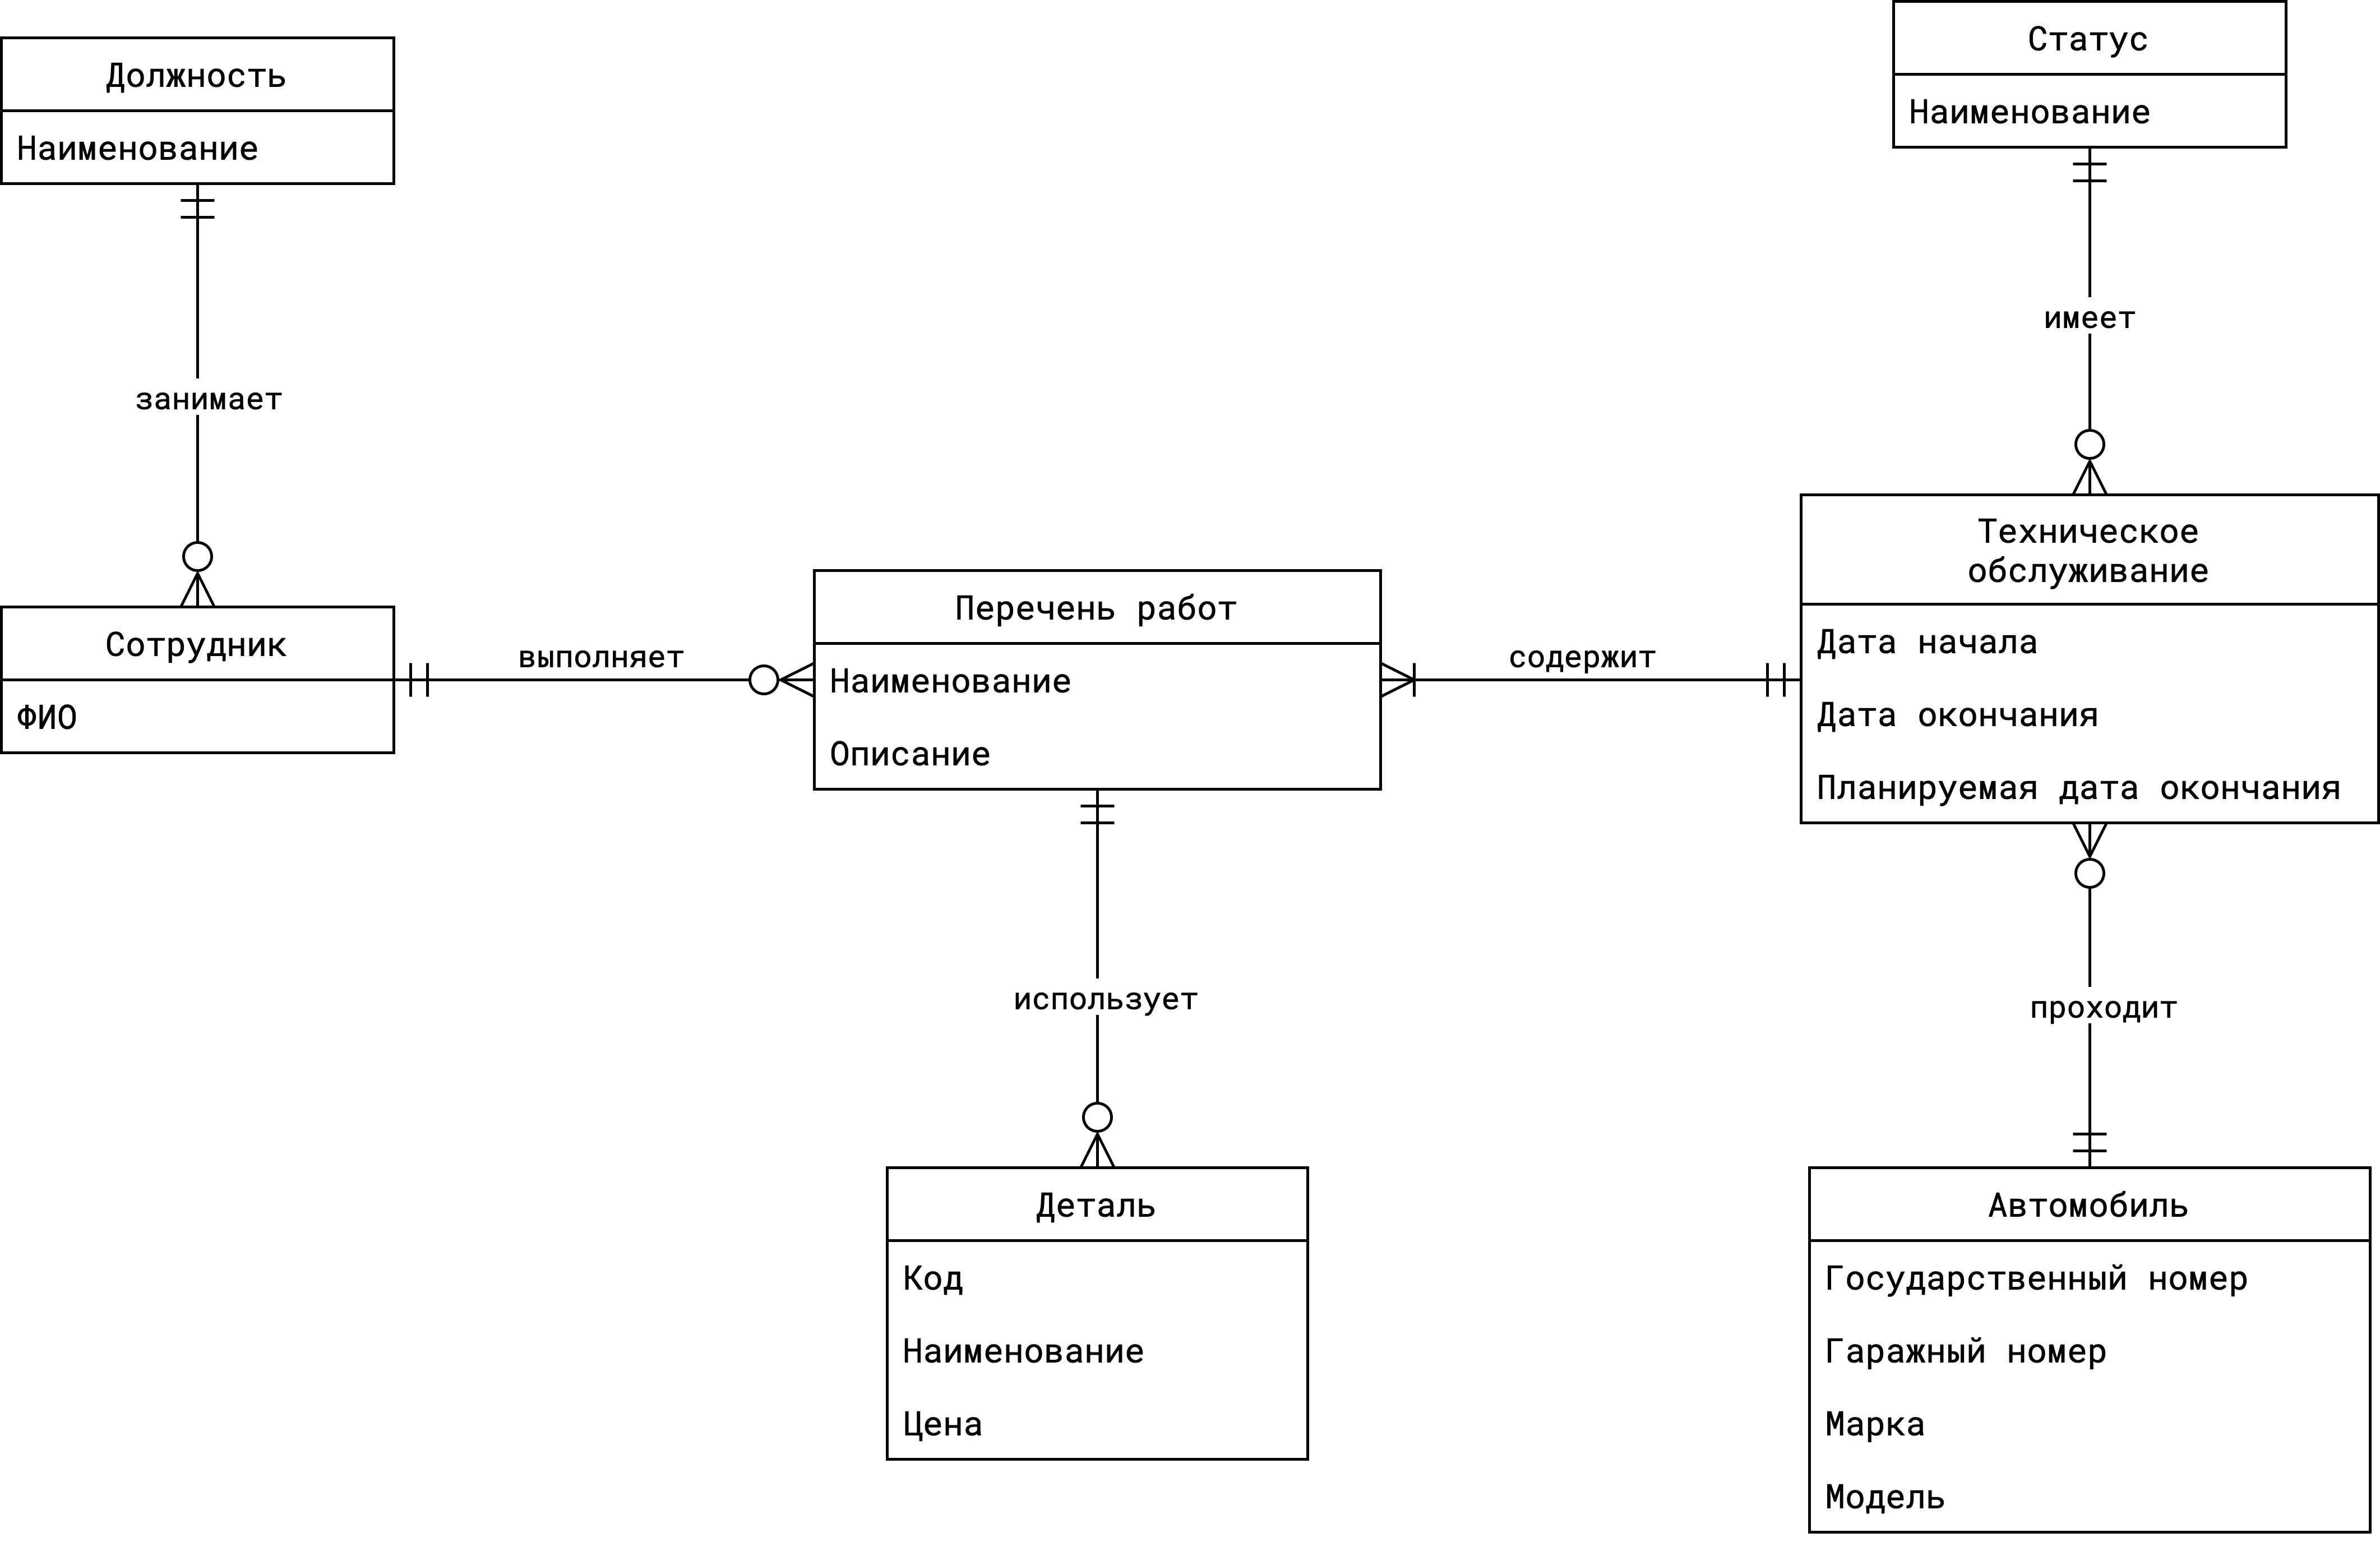
\includegraphics[keepaspectratio,width=\textwidth]{presentation/images/er-diagram.png}
        \label{fig:er-diagram}
    \end{figure}
\end{frame}

\begin{frame}
	{Теоретические математические модели}
    Стратегия для профилактируемых отказов и неисправностей
    \begin{equation*}
        d_{\text{п}} = d_{\text{к}} + k d_{\text{и}}\,,
    \end{equation*}
    {\footnotesize
        где $d_{\text{п}}$ -- стоимость ТО (профилактики); $d_{\text{к}}$ --
        стоимость контрольно-диагностической части операции ТО; $k$ --
        коэффициент повторяемости исполнительской части операции ТО;
        $d_{\text{и}}$ -- стоимость исполнительской части операции ТО.
    }
    \\[\baselineskip]
    Стратегия для непрофилактируемых отказов и неисправностей
    \begin{equation*}
        C^{II} =
        c\,/\,\bar{x} =
        c : \int_{x_{min}}^{x_{max}} x f(x)\,dx,
    \end{equation*}
    {\footnotesize
        где $\bar{x},\,x_{min} \,\text{и} \,x_{max}$ -- соответственно средняя,
        минимальная и максимальная наработки на отказ; $c$ -- разовые затраты на
        устранение отказа; $f(x)$ -- плотность вероятности наработки на отказ.
    }
\end{frame}

\begin{frame}
	{Эмпирические математические модели}
    \begin{columns}[c]
        \begin{column}{0.56\linewidth}
            \begin{figure}[h]
                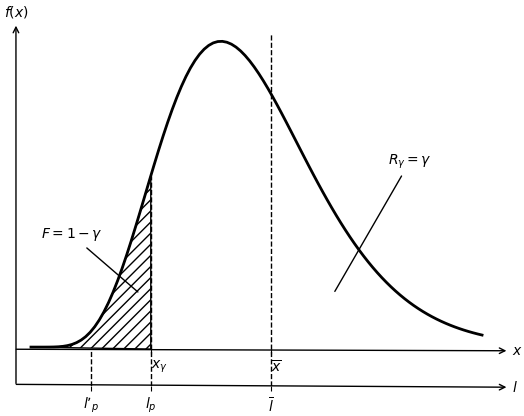
\includegraphics[keepaspectratio,width=\linewidth]{2/images/pdf.b.png}
            \end{figure}
        \end{column}
        \begin{column}{0.56\linewidth}
{\footnotesize
\begin{math}
    \arraycolsep=1.5pt\def\arraystretch{2.5}
    \begin{array}{l}
        \text{Пусть:}
        \begin{cases}
            d_\text{П} = d_\text{И}, \\
            x_{min} < l_p < \overline{x}
        \end{cases} \\

        l`_p = \left.
            \int_{x_{min}}^{l_p} lf(l)\,dl
        \middle/
            \left( \int_{x_{min}}^{l_p} f(l)\,dl \right)
        \right. \hfill (1) \\

        C^I_1 = \frac{cF + d_\Pi R}{l_p R + l`_p F} \hfill (2) \\

        C^I_2 = \frac%
            {cF + \left( d_K + d_\text{И} \right) R_1 + d_K R_2}%
            {l`_p F + l_p R}
        =
        \frac%
            {cF + R \left( d_K + d_\text{И} \right)}%
            {l`_p F + l_p R} \hfill (3) \\

        \left[
            \frac%
                { 2 k_\Pi \upsilon_x }%
                { \left( 1 + \upsilon^2_x \right) \left( 1 - \upsilon_x \right) }
        \right]^{ \upsilon_x }
        -
        \frac%
            { k_\Pi \upsilon_x }%
            { \left( 1 - \upsilon_x \right) }
        -
        k_\Pi > 0 \hfill (4)
    \end{array}
\end{math}
}
        \end{column}
    \end{columns}
\end{frame}

\begin{frame}
	{Логическая модель данных}
    \begin{figure}[H]
        \centering
        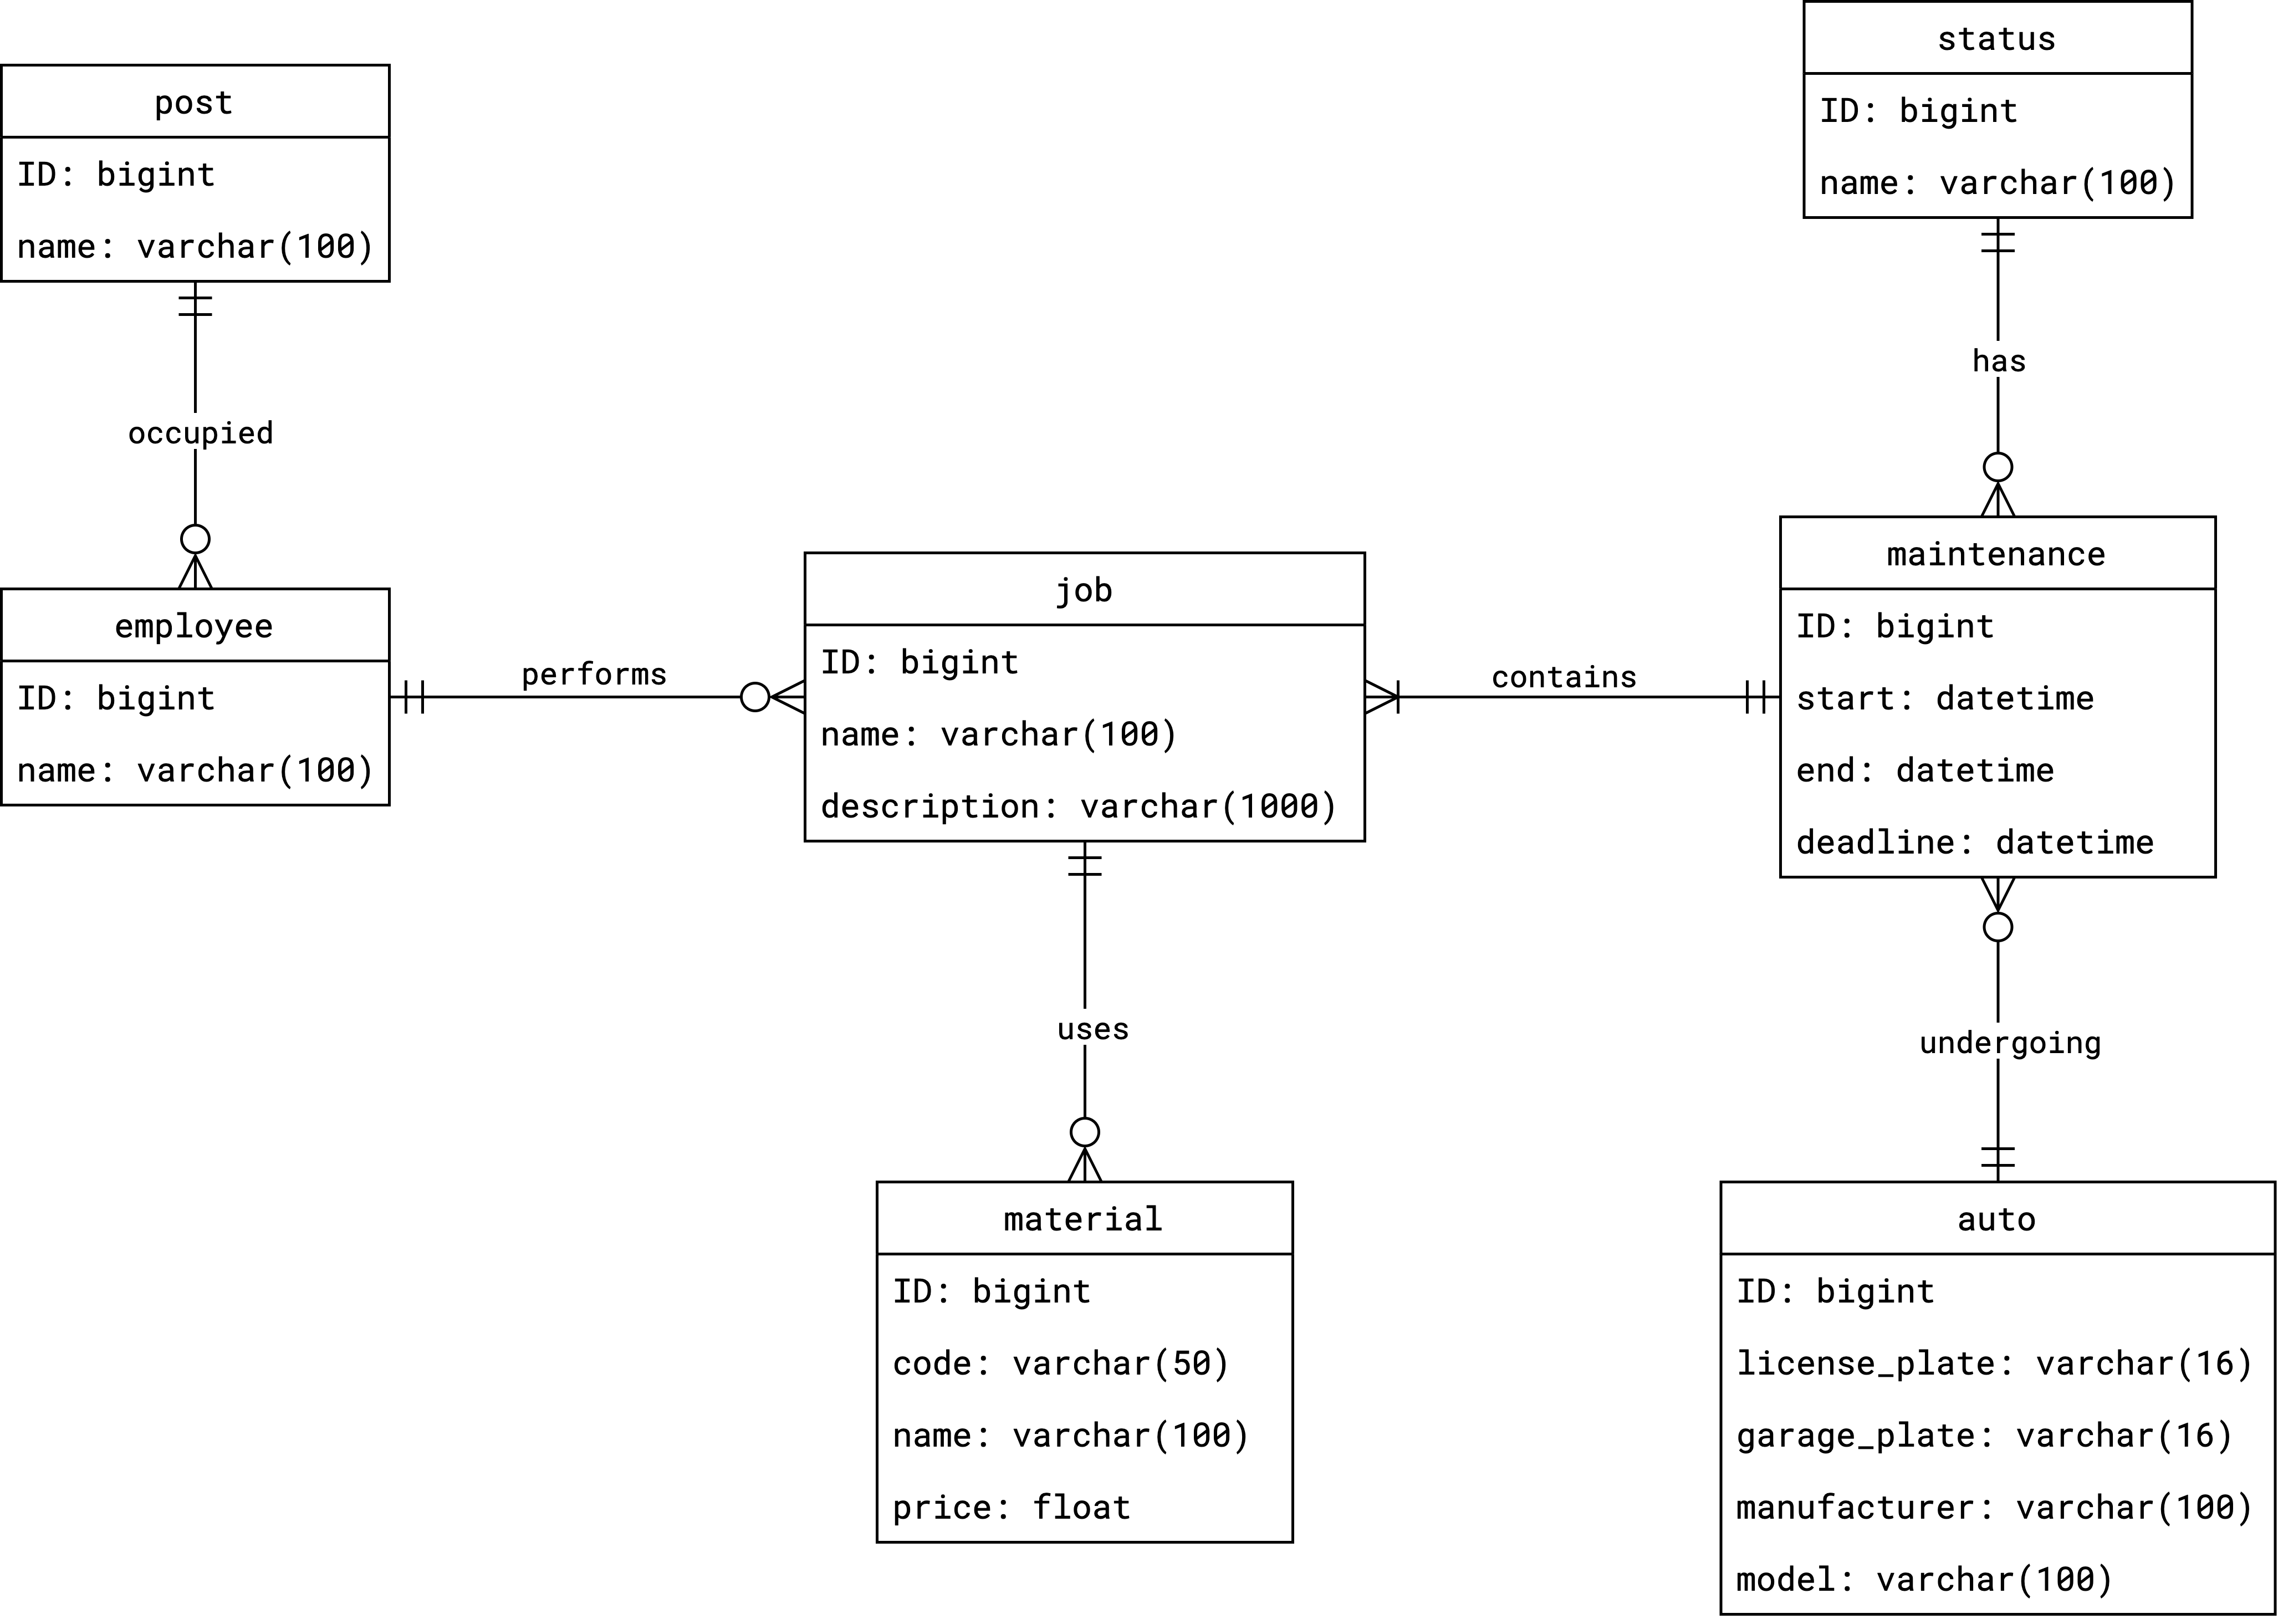
\includegraphics[keepaspectratio,width=\textwidth]{3/images/3_1_db_logical.png}
    \end{figure}
\end{frame}

\begin{frame}
	{Физическая модель данных}
    \begin{figure}[H]
        \centering
        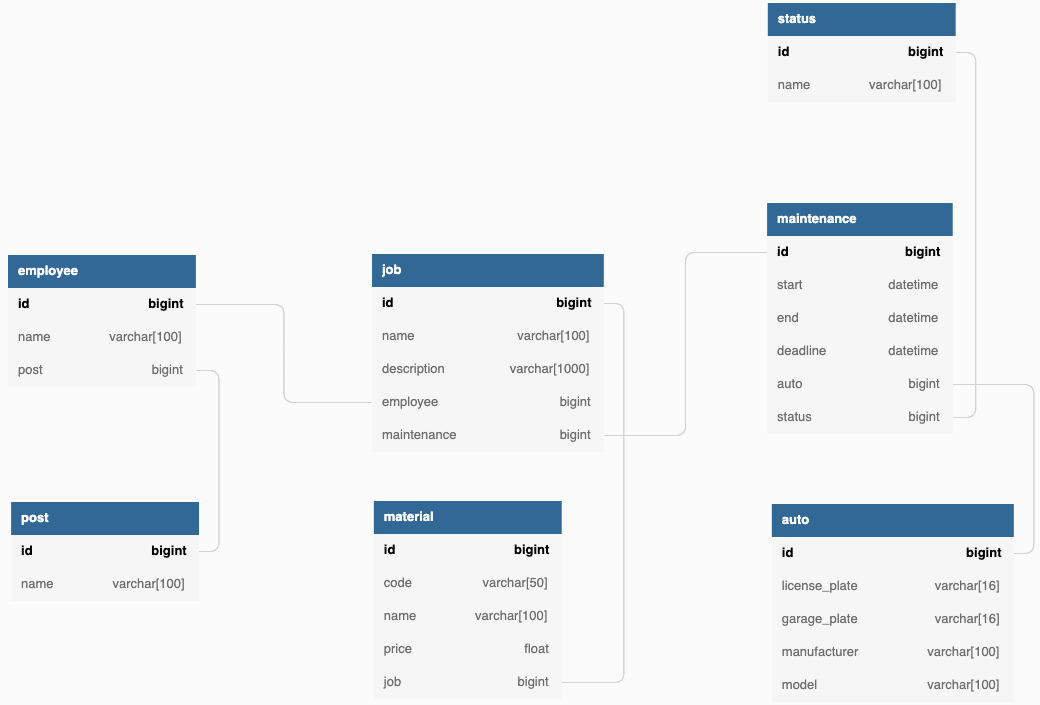
\includegraphics[keepaspectratio,width=\textwidth]{3/images/3_1_db_physical.png}
    \end{figure}
\end{frame}

\begin{frame}
	{Описание источников информации, входных сигналов и документов}
    Основными источниками информации в системе являются:
    \begin{enumerate}
        \item Входные данные пользователей системы, полученные от администратора,
            при их регистрации в системе.
        \item Входные данные техники, полученные от старшего техника, при их
            регистрации в системе.
        \item Информация о необходимых материалах для проведения технического
            обслуживания и ремонта автомобиля.
    \end{enumerate}
\end{frame}

\begin{frame}
	{Описание выходной информации: сигналов, документов и видеокадров}
    График прохождения технического осмотра.
    \begin{figure}[H]
        \centering
        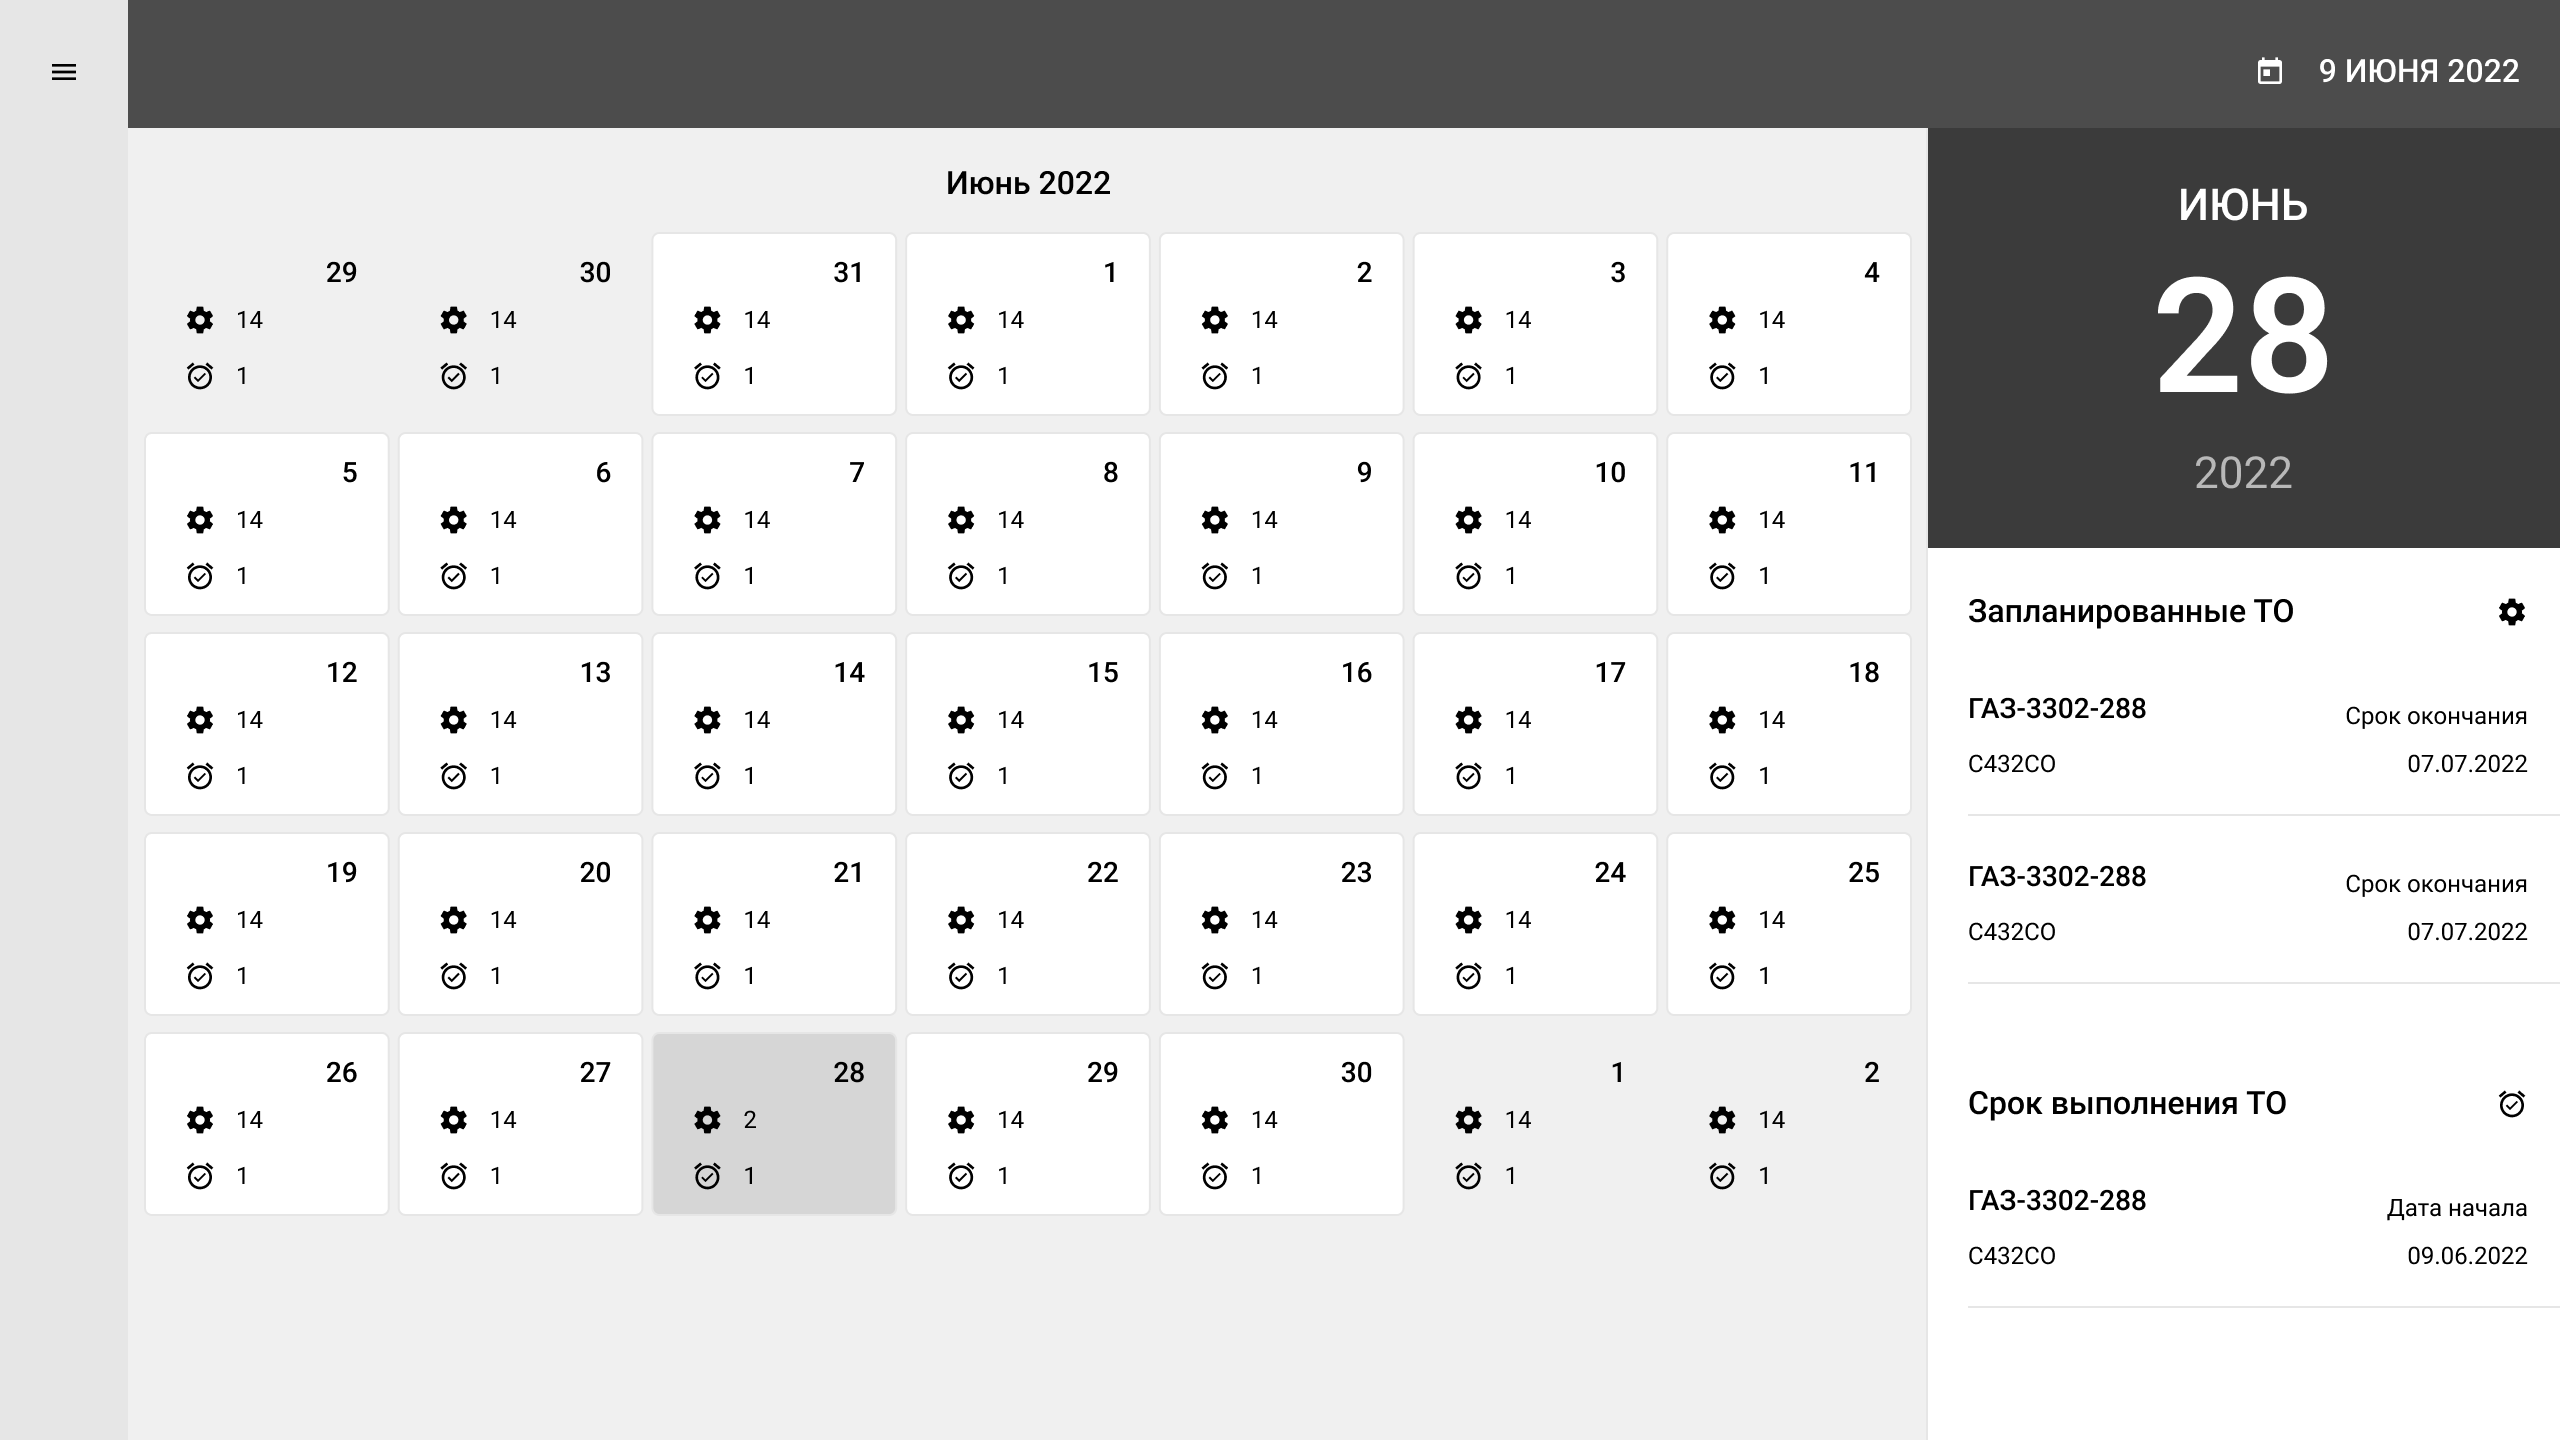
\includegraphics[keepaspectratio,width=\textwidth]{3/images/calendar-planning.png}
    \end{figure}
\end{frame}
\begin{frame}
	{Описание выходной информации: сигналов, документов и видеокадров}
    Отчеты по затратам
    \begin{figure}[H]
        \centering
        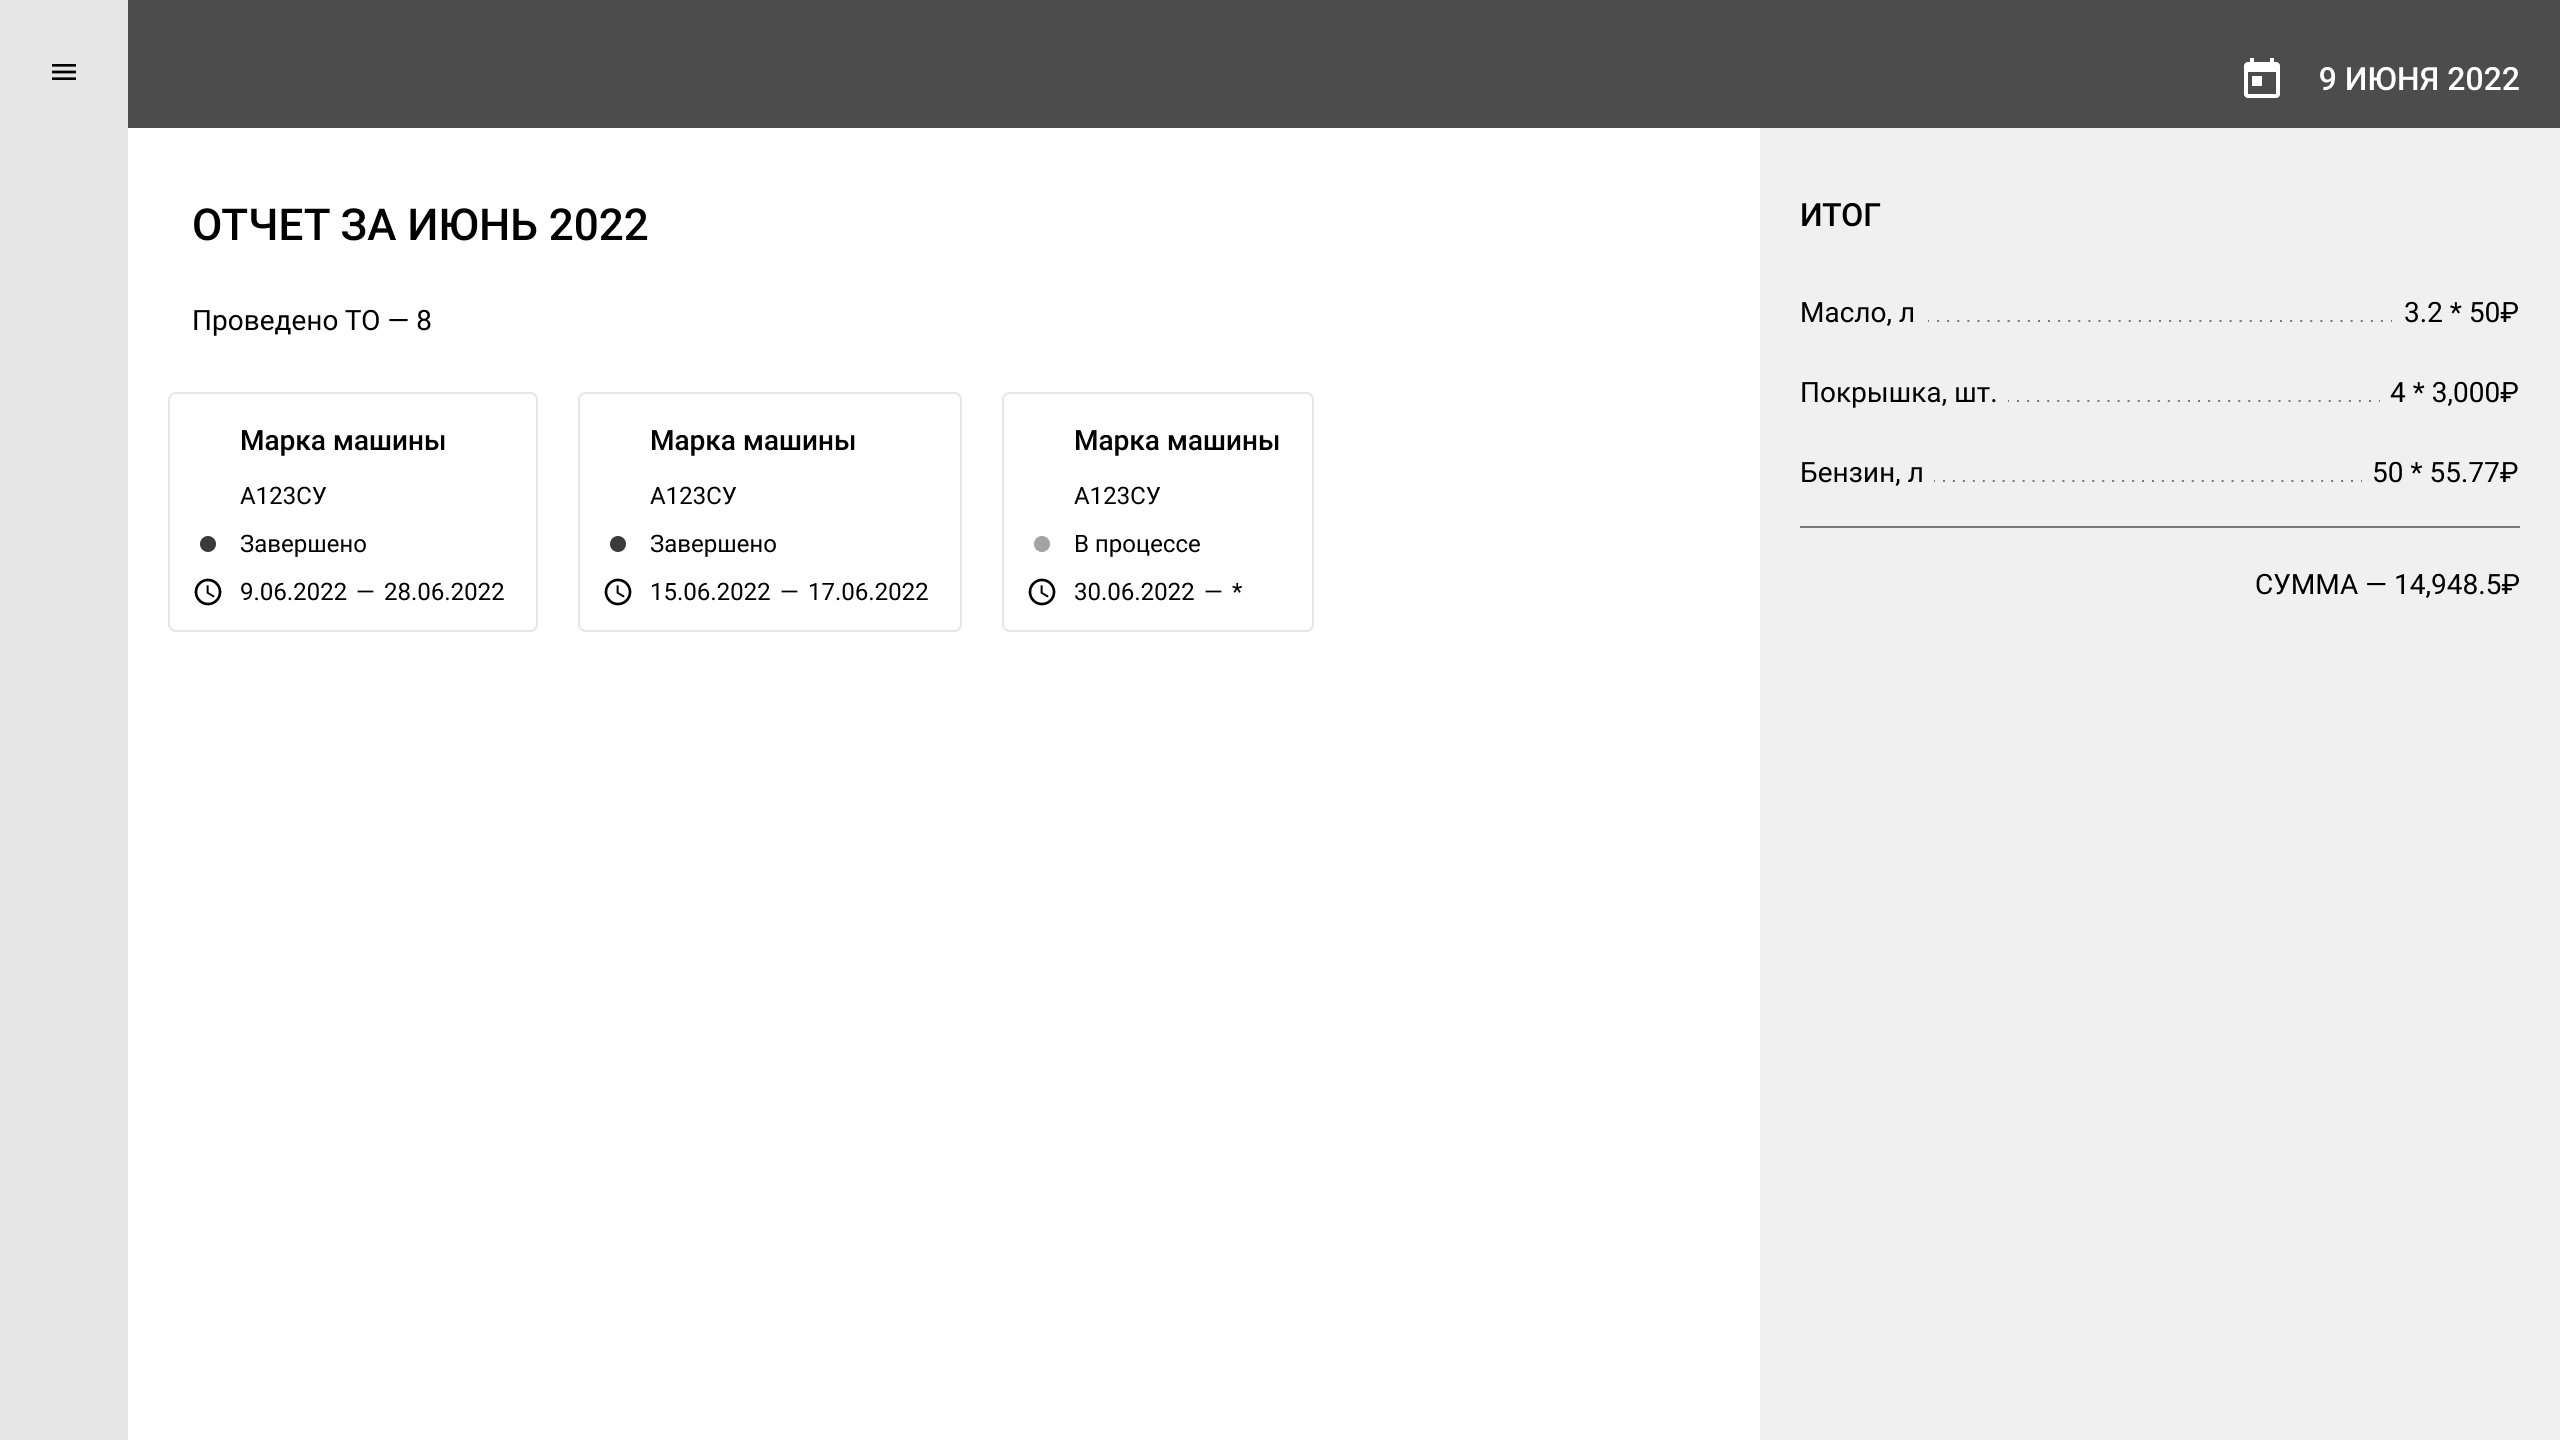
\includegraphics[keepaspectratio,width=\textwidth]{3/images/expenses-report.png}
    \end{figure}
\end{frame}

\end{document}
